% Generado por floyd.c
\documentclass[a4paper,11pt]{article}
\usepackage[utf8]{inputenc}
\usepackage{tikz}
\usepackage{array}
\usepackage[table]{xcolor}
\usepackage{longtable}
\usepackage{geometry}
\geometry{margin=1.5cm}
\begin{document}
\begin{center}
{\LARGE \textbf{Proyecto 1: Algoritmo de Floyd}}\\[2cm]
{\large Investigacion de Operaciones\\[2cm]
{\large Integrantes: }\\[1cm]
{\large Jose Pablo Fernandez Jimenez - 2023117752}\\[1cm]
{\large Diego Duran Rodriguez - 2022437509}\\[2cm]
{\large Segundo semestre 2025\\[1cm]
\end{center}
\newpage
\section*{Algoritmo de Floyd}
Descripcion

\bigskip
\section*{Problema}
\begin{center}
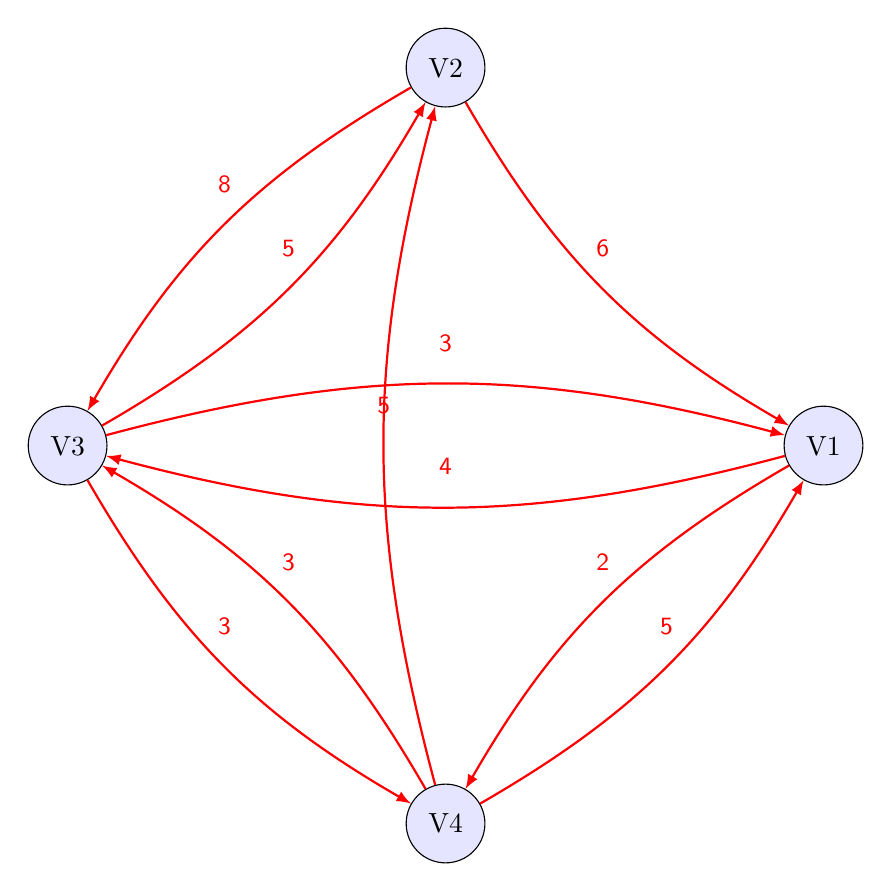
\begin{tikzpicture}[scale=1.2,
  every node/.style={circle, draw, fill=blue!10, minimum size=10mm},
  every edge/.style={draw, thick}]
\node (N0) at (4.000, 0.000) {V1};
\node (N1) at (0.000, 4.000) {V2};
\node (N2) at (-4.000, 0.000) {V3};
\node (N3) at (-0.000, -4.000) {V4};
\draw[->, thick, >=latex, red] (N0) to[bend left=15] node[midway, above, draw=none, fill=none, rectangle, font=\small\sffamily] {4} (N2);
\draw[->, thick, >=latex, red] (N0) to[bend right=15] node[midway, above, draw=none, fill=none, rectangle, font=\small\sffamily] {2} (N3);
\draw[->, thick, >=latex, red] (N1) to[bend right=15] node[midway, above, draw=none, fill=none, rectangle, font=\small\sffamily] {6} (N0);
\draw[->, thick, >=latex, red] (N1) to[bend right=15] node[midway, above, draw=none, fill=none, rectangle, font=\small\sffamily] {8} (N2);
\draw[->, thick, >=latex, red] (N2) to[bend left=15] node[midway, above, draw=none, fill=none, rectangle, font=\small\sffamily] {3} (N0);
\draw[->, thick, >=latex, red] (N2) to[bend right=15] node[midway, above, draw=none, fill=none, rectangle, font=\small\sffamily] {5} (N1);
\draw[->, thick, >=latex, red] (N2) to[bend right=15] node[midway, above, draw=none, fill=none, rectangle, font=\small\sffamily] {3} (N3);
\draw[->, thick, >=latex, red] (N3) to[bend right=15] node[midway, above, draw=none, fill=none, rectangle, font=\small\sffamily] {5} (N0);
\draw[->, thick, >=latex, red] (N3) to[bend left=15] node[midway, above, draw=none, fill=none, rectangle, font=\small\sffamily] {5} (N1);
\draw[->, thick, >=latex, red] (N3) to[bend right=15] node[midway, above, draw=none, fill=none, rectangle, font=\small\sffamily] {3} (N2);
\end{tikzpicture}
\end{center}
\newpage
\section*{Tablas iniciales}
\subsection*{D(0)}
\begin{center}
\begin{tabular}{c|cccc}
 & V1 & V2 & V3 & V4 \\ \hline
V1 & 0 & $\infty$ & 4 & 2 \\
V2 & 6 & 0 & 8 & $\infty$ \\
V3 & 3 & 5 & 0 & 3 \\
V4 & 5 & 5 & 3 & 0 \\
\end{tabular}
\end{center}
\subsection*{P(0)}
\begin{center}
\begin{tabular}{c|cccc}
 & V1 & V2 & V3 & V4 \\ \hline
V1 & 0 & 0 & 0 & 0 \\
V2 & 0 & 0 & 0 & 0 \\
V3 & 0 & 0 & 0 & 0 \\
V4 & 0 & 0 & 0 & 0 \\
\end{tabular}
\end{center}
\newpage
\section*{Tablas intermedias}
\section*{Calculo de D(1)}
\subsection*{D(1)}
\begin{center}
\begin{tabular}{c|cccc}
 & V1 & V2 & V3 & V4 \\ \hline
V1 & 0 & $\infty$ & 4 & 2 \\
V2 & 6 & 0 & 8 & \textcolor{orange}{8} \\
V3 & 3 & 5 & 0 & 3 \\
V4 & 5 & 5 & 3 & 0 \\
\end{tabular}
\end{center}
\subsection*{P(1)}
\begin{center}
\begin{tabular}{c|cccc}
 & V1 & V2 & V3 & V4 \\ \hline
V1 & - & - & - & - \\
V2 & - & - & - & V1 \\
V3 & - & - & - & - \\
V4 & - & - & - & - \\
\end{tabular}
\end{center}
\newpage
\section*{Calculo de D(2)}
\subsection*{D(2)}
\begin{center}
\begin{tabular}{c|cccc}
 & V1 & V2 & V3 & V4 \\ \hline
V1 & 0 & $\infty$ & 4 & 2 \\
V2 & 6 & 0 & 8 & 8 \\
V3 & 3 & 5 & 0 & 3 \\
V4 & 5 & 5 & 3 & 0 \\
\end{tabular}
\end{center}
\subsection*{P(2)}
\begin{center}
\begin{tabular}{c|cccc}
 & V1 & V2 & V3 & V4 \\ \hline
V1 & - & - & - & - \\
V2 & - & - & - & V1 \\
V3 & - & - & - & - \\
V4 & - & - & - & - \\
\end{tabular}
\end{center}
\newpage
\section*{Calculo de D(3)}
\subsection*{D(3)}
\begin{center}
\begin{tabular}{c|cccc}
 & V1 & V2 & V3 & V4 \\ \hline
V1 & 0 & \textcolor{orange}{9} & 4 & 2 \\
V2 & 6 & 0 & 8 & 8 \\
V3 & 3 & 5 & 0 & 3 \\
V4 & 5 & 5 & 3 & 0 \\
\end{tabular}
\end{center}
\subsection*{P(3)}
\begin{center}
\begin{tabular}{c|cccc}
 & V1 & V2 & V3 & V4 \\ \hline
V1 & - & V3 & - & - \\
V2 & - & - & - & V1 \\
V3 & - & - & - & - \\
V4 & - & - & - & - \\
\end{tabular}
\end{center}
\newpage
\section*{Calculo de D(4)}
\subsection*{D(4)}
\begin{center}
\begin{tabular}{c|cccc}
 & V1 & V2 & V3 & V4 \\ \hline
V1 & 0 & \textcolor{orange}{7} & 4 & 2 \\
V2 & 6 & 0 & 8 & 8 \\
V3 & 3 & 5 & 0 & 3 \\
V4 & 5 & 5 & 3 & 0 \\
\end{tabular}
\end{center}
\subsection*{P(4)}
\begin{center}
\begin{tabular}{c|cccc}
 & V1 & V2 & V3 & V4 \\ \hline
V1 & - & V4 & - & - \\
V2 & - & - & - & V1 \\
V3 & - & - & - & - \\
V4 & - & - & - & - \\
\end{tabular}
\end{center}
\newpage
\section*{Distancias y rutas \'optimas}
\begin{longtable}{c c c p{7cm}}
\hline
Origen & Destino & Distancia & Ruta \\\hline
\endhead
V1 & V2 & 7 & V1 -- V4 -- V2 \\
V1 & V3 & 4 & V1 -- V3 \\
V1 & V4 & 2 & V1 -- V4 \\
V2 & V1 & 6 & V2 -- V1 \\
V2 & V3 & 8 & V2 -- V3 \\
V2 & V4 & 8 & V2 -- V1 -- V4 \\
V3 & V1 & 3 & V3 -- V1 \\
V3 & V2 & 5 & V3 -- V2 \\
V3 & V4 & 3 & V3 -- V4 \\
V4 & V1 & 5 & V4 -- V1 \\
V4 & V2 & 5 & V4 -- V2 \\
V4 & V3 & 3 & V4 -- V3 \\
\hline
\end{longtable}
\end{document}
